% A LaTeX (non-official) template for ISAE projects reports
% Copyright (C) 2014 Damien Roque
% Version: 0.2
% Author: Damien Roque <damien.roque_AT_isae.fr>

\documentclass[a4paper,10pt,calibri,oneside,openany, twocolumn]{report}
\usepackage{geometry}
\setlength{\voffset}{-0.75in}
\setlength{\headsep}{5pt}
\usepackage[utf8]{inputenc}
\usepackage[T1]{fontenc}
%\usepackage[french]{babel} % If you write in French
\usepackage[english]{babel} % If you write in English
\usepackage{a4wide}
\usepackage{graphicx}
\graphicspath{{images/}}
\usepackage{subfig}
\usepackage{tikz}
\usetikzlibrary{shapes,arrows}
\usepackage{pgfplots}
\pgfplotsset{compat=newest}
\pgfplotsset{plot coordinates/math parser=false}
\newlength\figureheight
\newlength\figurewidth
\pgfkeys{/pgf/number format/.cd,
set decimal separator={,\!},
1000 sep={\,},
}
\usepackage{ifthen}
\usepackage{ifpdf}
\usepackage{pdfpages}
\ifpdf
\usepackage[pdftex]{hyperref}
\else
\usepackage{hyperref}
\fi
\usepackage{color}
\hypersetup{%
colorlinks=true,
linkcolor=black,
citecolor=black,
urlcolor=black}
\usepackage{float}
\renewcommand{\baselinestretch}{1.05}
\usepackage{fancyhdr}
\pagestyle{fancy}
\fancyfoot{}
\fancyhead[C]{Recherche opérationnelle}
\fancyhead[L]{SM2}
\fancyhead[R]{TP2 - US Elections 2016}
\usepackage{colortbl}
\arrayrulecolor{black}


\usepackage{lastpage}
\renewcommand\headrulewidth{1pt}
\fancyfoot[L]{PORET, HUYNH}
\renewcommand\footrulewidth{1pt}
\fancyfoot[C]{\textbf{Page \thepage/\pageref{LastPage}}}
\fancyfoot[R]{\today}
\makeatletter
\def\@textbottom{\vskip \z@ \@plus 1pt}
\let\@texttop\relax
\makeatother

\makeatletter
\def\cleardoublepage{\clearpage\if@twoside \ifodd\c@page\else%
  \hbox{}%
  \thispagestyle{empty}%
  \newpage%
  \if@twocolumn\hbox{}\newpage\fi\fi\fi}
\makeatother
\usepackage{makecell}
\usepackage{amsthm}
\usepackage{amssymb,amsmath,bbm}
\usepackage{array}
\usepackage{bm}
\usepackage{multirow}
\usepackage[footnote]{acronym}
\usepackage{float}
\usepackage{wasysym}
\usepackage{wrapfig}
\usepackage{url}
\usepackage{eurosym}
\usepackage{array}
\usepackage{xcolor}
\usepackage{supertabular}
\usepackage{pdflscape}
\usepackage{calrsfs}
\usepackage{longtable, booktabs}
\usepackage{minted}
\newcommand*{\SET}[1]  {\ensuremath{\mathbf{#1}}}
\newcommand*{\VEC}[1]  {\ensuremath{\boldsymbol{#1}}}
\newcommand*{\FAM}[1]  {\ensuremath{\boldsymbol{#1}}}
\newcommand*{\MAT}[1]  {\ensuremath{\boldsymbol{#1}}}
\newcommand*{\OP}[1]  {\ensuremath{\mathrm{#1}}}
\newcommand*{\NORM}[1]  {\ensuremath{\left\|#1\right\|}}
\newcommand*{\DPR}[2]  {\ensuremath{\left \langle #1,#2 \right \rangle}}
\newcommand*{\calbf}[1]  {\ensuremath{\boldsymbol{\mathcal{#1}}}}
\newcommand*{\shift}[1]  {\ensuremath{\boldsymbol{#1}}}
\addto\extrasenglish{%
  \renewcommand{\chapterautorefname}{Chapter}%
}
\newcommand{\eqdef}{\stackrel{\mathrm{def}}{=}}
\newcommand{\argmax}{\operatornamewithlimits{argmax}}
\newcommand{\argmin}{\operatornamewithlimits{argmin}}
\newcommand{\ud}{\, \mathrm{d}}
\newcommand{\vect}{\text{Vect}}
\newcommand{\sinc}{\ensuremath{\mathrm{sinc}}}
\newcommand{\esp}{\ensuremath{\mathbb{E}}}
\newcommand{\hilbert}{\ensuremath{\mathcal{H}}}
\newcommand{\fourier}{\ensuremath{\mathcal{F}}}
\newcommand{\sgn}{\text{sgn}}
\newcommand{\intTT}{\int_{-T}^{T}}
\newcommand{\intT}{\int_{-\frac{T}{2}}^{\frac{T}{2}}}
\newcommand{\intinf}{\int_{-\infty}^{+\infty}}
\newcommand{\Sh}{\ensuremath{\boldsymbol{S}}}
\newcommand{\C}{\SET{C}}
\newcommand{\R}{\SET{R}}
\newcommand{\Z}{\SET{Z}}
\newcommand{\N}{\SET{N}}
\newcommand{\K}{\SET{K}}
\newcommand{\reel}{\mathcal{R}}
\newcommand{\imag}{\mathcal{I}}
\newcommand{\cmnr}{c_{m,n}^\reel}
\newcommand{\cmni}{c_{m,n}^\imag}
\newcommand{\cnr}{c_{n}^\reel}
\newcommand{\cni}{c_{n}^\imag}
\newcommand{\tproto}{g}
\newcommand{\rproto}{\check{g}}
\newcommand{\LR}{\mathcal{L}_2(\SET{R})}
\newcommand{\LZ}{\ell_2(\SET{Z})}
\newcommand{\LZI}[1]{\ell_2(\SET{#1})}
\newcommand{\LZZ}{\ell_2(\SET{Z}^2)}
\newcommand{\diag}{\operatorname{diag}}
\newcommand{\noise}{z}
\newcommand{\Noise}{Z}
\newcommand{\filtnoise}{\zeta}
\newcommand{\tp}{g}
\newcommand{\rp}{\check{g}}
\newcommand{\TP}{G}
\newcommand{\RP}{\check{G}}
\newcommand{\dmin}{d_{\mathrm{min}}}
\newcommand{\Dmin}{D_{\mathrm{min}}}
\newcommand{\Image}{\ensuremath{\text{Im}}}
\newcommand{\Span}{\ensuremath{\text{Span}}}

\newcommand{\anfr}[1]{{\bfseries\underline{#1}}}

\newtheoremstyle{break}
  {11pt}{11pt}%
  {\itshape}{}%
  {\bfseries}{}%
  {\newline}{}%
\theoremstyle{break}

%\theoremstyle{definition}
\newtheorem{definition}{Définition}[chapter]

%\theoremstyle{definition}
\newtheorem{theoreme}{Théorème}[chapter]

%\theoremstyle{remark}
\newtheorem{remarque}{Remarque}[chapter]

%\theoremstyle{plain}
\newtheorem{propriete}{Propriété}[chapter]
\newtheorem{exemple}{Exemple}[chapter]



%\sloppy
\usepackage{multicol}
\usepackage{wrapfig}
\usepackage{enumitem}
\usepackage{pifont}
\usepackage{makeidx}
\usepackage{setspace}
\usepackage{xr}
\usepackage{zref}
\usepackage{zref-xr}
\usepackage{xr-hyper}
\setlength{\columnsep}{1.5cm}
\setlength{\columnseprule}{0.2pt}
\makeindex
\usepackage[xindy]{glossaries}
\usepackage{adjustbox}
\makeglossaries
\usepackage{lipsum}
%\loadglsentries{glossaire.tex}




\begin{document}


	\begin{center}
		\bfseries TP 2 - Members in the US\\ Electoral College
	\end{center}
\section*{General information}
Population data is from 2016. We chose to use the eligible population as it is more representative of the 2016 Elections.\\

The US' rules about their Electoral College are rather complicated and the first one we should mention is specific to the 2016 Elections as Puerto Rico was not allowed to take part in the voting process as it is seen as a territory and not a state.\\

Some other very specific rules include the distribution of members of the Electoral College within a state because of how those are made out of lower level territorial decomposition. For example
\section*{Linear Programming problem}
\begin{equation}
\begin{cases}
min\ u-v& \\
v - \frac{\alpha_i}{x_i}&\leq 0\\
\frac{\alpha_i}{x_i}- u &\leq 0\\
\sum\limits_i \alpha_i &= N
\end{cases}
\end{equation}
This LP problem is acts a bit like a dichotomy. By minimizing our objective function $u-v$ which are tool variables, while keeping $u>v$, will diminish the interval where $\frac{\alpha_i}{x_i}$ can be as it is "sandwiching" it. This ratio between the members at the Electoral College and the eligible population for each state is important. Indeed, if for each state, having a small interval for those ratios, meaning that all ratios are nearby one another for every given state will insure that the number of members in the Electoral College is well and evenly spread accordingly to the population of that state.\\

The last constraint is also extremely important as it keeps the sum of those members to that given $N=538$ in the US constitution. The solutions $\alpha_i$ of this LP problem will give us the best distribution of Electoral College seats while focusing \textbf{ONLY} on the number of eligible voters per state and the number of available seats. \\

Other discussions could be made about some other constraints such as adding a minimal number of seats per state (it is currently 3 by US Constitution) but we noticed that even without that constraint, no state has $0$ seats. In order to make it as fair as possible and to avoid large discrepancies between states, we decided to consider to not take the current minimal 3 seats condition into account as this will create a larger variation in seats for states while having a small change in population.
\section*{Results and optimization}
\qquad With our problem as stated before, we have a rather disturbing problem as we can see that some states have fairly similar populations but sometimes have double the members in the electoral college. This is particularly obvious when we took at the lower end of the population spectrum where there isn't a lot of population but we might see. For example, with our first LP, Vermont had a ratio $\frac{\alpha_{Vermont}}{x_{Vermont}}\times10^6=4.041$ while California had $\frac{\alpha_{California}}{x_{California}}\times10^6=2.151$. This is due to a matrix conditioning problem when working on the LP problem as the orders of magnitude vary greatly between $10^{-6}\ (u,\ v)$, $10^0\ (\alpha_i)$ and $10^6\ (x_i)$.\\

Thus, our problem has been slightly modified to :
\begin{equation}
	\begin{cases}
	min\ u-v& \\
	v - \frac{\alpha_i}{x_i}\times 10^6&\leq 0\\
	\frac{\alpha_i}{x_i}\times 10^6 - u &\leq 0\\
	\sum\limits_i \alpha_i &= N
	\end{cases}
\end{equation}
By doing this, we will do some kind of pre-conditioning which will make our results better. With this change, the number of members per state is given by :
\begin{table}
	\begin{tabular}{|c|c|c|c|}
	\hline
	\cellcolor{gray!30} State & \cellcolor{gray!30} \shortstack{Voting \\Population}&\cellcolor{gray!30}\shortstack{Members in\\ Electoral C.}&\cellcolor{gray!30}$\frac{\alpha_i\times 10^6}{x_i}$\\
	\hline
	Alabama &3 609 447&9&2.493\\
	\hline
	Alaska &522 679&1&1.913\\
	\hline
	Arizona &4 740 310 &12&2.531\\
	\hline
	Arkansas &2 140 097&5&2.336\\
	\hline
	California &25 104 844&49&1.952\\
	\hline
	Colorado &3 974 405&10&2.516\\
	\hline
	Connecticut &2 582 761&6&2.323\\
	\hline
	Delaware &691 720&1&1.446\\
	\hline
	DC &515 248&1&1.941\\
	\hline
	Florida &14 601 066&37&2.534\\
	\hline
	Georgia &6 959 963&17&2.443\\
	\hline
	Hawaii &1 012 860&2&1.975\\
	\hline
	Idaho &1 166 706&2&1.714\\
	\hline
	Illinois &8 985 443&22&2.448\\
	\hline
	Indiana &4 849 937&12&2.474\\
	\hline
	Iowa &2 288 536&5&2.185\\
	\hline
	Kansas &2 054 025&5&2.434\\
	\hline
	Kentucky &3 282 420&8&2.437\\
	\hline
	Louisiana &3 384 435&8&2.364\\
	\hline
	Maine &1 058 372&2&1.890\\
	\hline
	Maryland &4 189 616&10&2.387\\
	\hline
	Massachusetts &4 948 028&12&2.425\\
	\hline
	Michigan &7 420 628&18&2.426\\
	\hline
	Minnesota &3 973 204&10&2.517\\
	\hline
	Mississippi &2 191 241&5&2.282\\
	\hline
	Missouri &4 517 925&11&2.435\\
	\hline
	Montana &804 250&2&2.487\\
	\hline
	Nebraska &1 343 821&3&2.232\\
	\hline
	Nevada &1 961 587&4&2.039\\
	\hline
	New Hampshire &1 042 795&2&1.918\\
	\hline
	New Jersey &6 013 656&15&2.494\\
	\hline
	New Mexico &1 464 515&3&2.048\\
	\hline
	New York &13 604 645&34&2.499\\
	\hline
	North Carolina &7 352 501&18&2.448\\
	\hline
	North Dakota &566 783&1&1.764\\
	\hline
	Ohio &8 736 808&22&2.518\\
	\hline
	Oklahoma &2 778 219&7&2.520\\
	\hline
	Oregon &3 024 174&7&2.315\\
	\hline
	Pennsylvania &9 691 160&24&2.476\\
	\hline
	Rhode Island &786 012&2&2.554\\
	\hline
	South Carolina &3 709 283&9&2.426\\
	\hline
	South Dakota &631 173&1&1.584\\
	\hline
	Tennessee &4 909 426&12&2.444\\
	\hline
	Texas &17 448 910&44&2.522\\
	\hline
	Utah &1 991 885&5&2.510\\
	\hline
	Vermont &494 871&1&2.021\\
	\hline
	Virginia &6 027 152&15&2.489\\
	\hline
	Washington &5 123 020&13&2.538\\
	\hline
	West Virginia &1 423 031&3&2.108\\
	\hline
	Wisconsin &4 285 071&10&2.334\\
	\hline
	Wyoming &429 682&1&2.327\\
	\hline
	\end{tabular}
\end{table}

\clearpage
\section*{US Maps}

\begin{figure}[H]
	\centering
	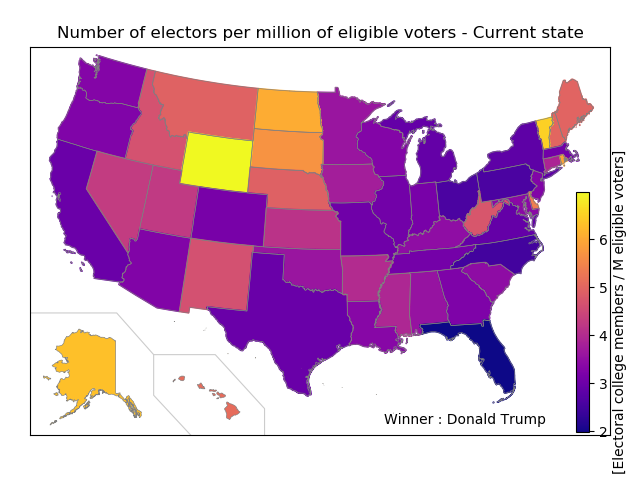
\includegraphics[width=\linewidth]{mapCurrentEligible}
	\caption{Current distribution : $\frac{\alpha_{real,eligible_i}}{x_i}$}
\end{figure}
\begin{figure}[H]
	\centering
	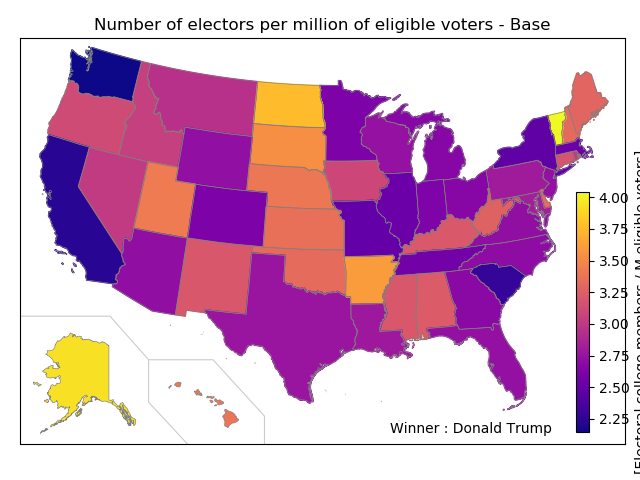
\includegraphics[width=\linewidth]{mapEligibleBase}
	\caption{Distribution without conditioning - Eligible voters only}
\end{figure}
\begin{figure}[H]
	\centering
	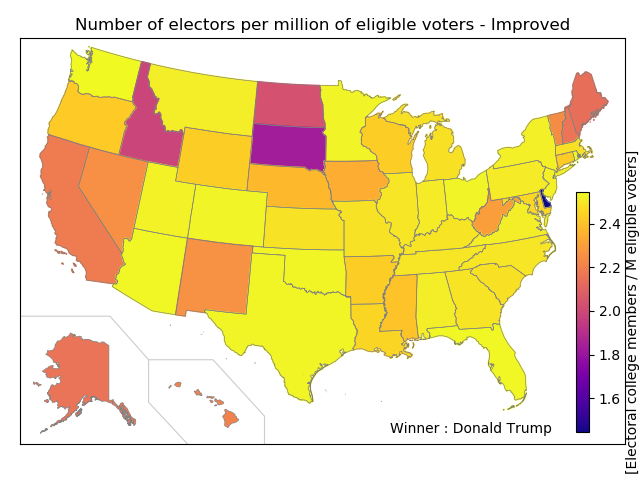
\includegraphics[width=\linewidth]{mapEligibleImproved}
	\caption{Distribution with conditioning - Eligible voters only}
\end{figure}

\begin{figure}[H]
	\vspace*{1.8cm}
	\centering
	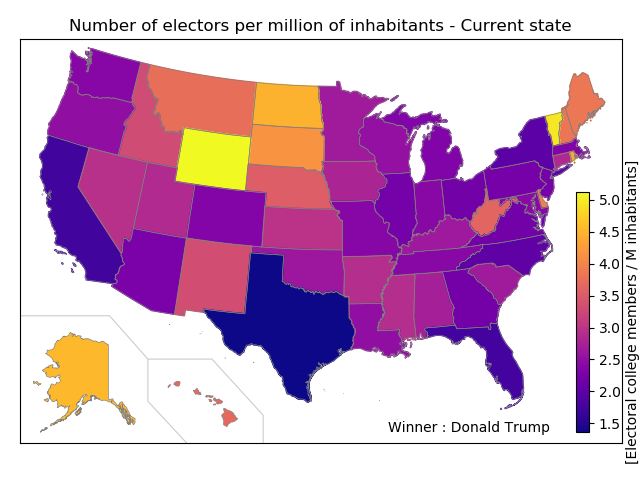
\includegraphics[width=\linewidth]{mapCurrentTotal}
	\caption{Current distribution : $\frac{\alpha_{real,total_i}}{x_i}$}
\end{figure}
\begin{figure}[H]
	\vspace*{0.3cm}

	\centering
	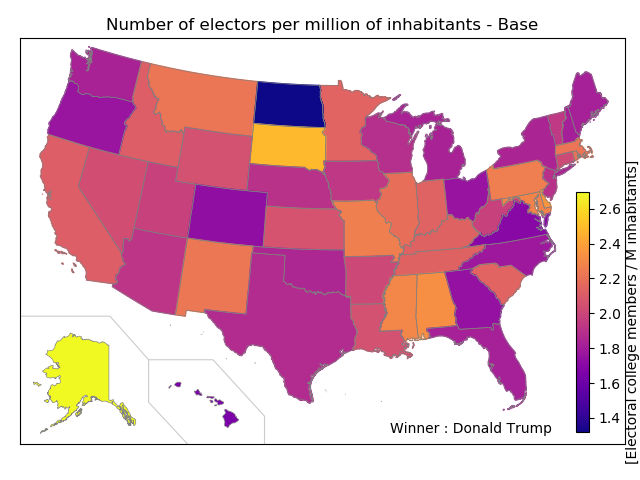
\includegraphics[width=\linewidth]{mapTotalBase}
	\caption{Distribution without conditioning - Whole population}
\end{figure}
\begin{figure}[H]
	\vspace*{0.5cm}
	\centering
	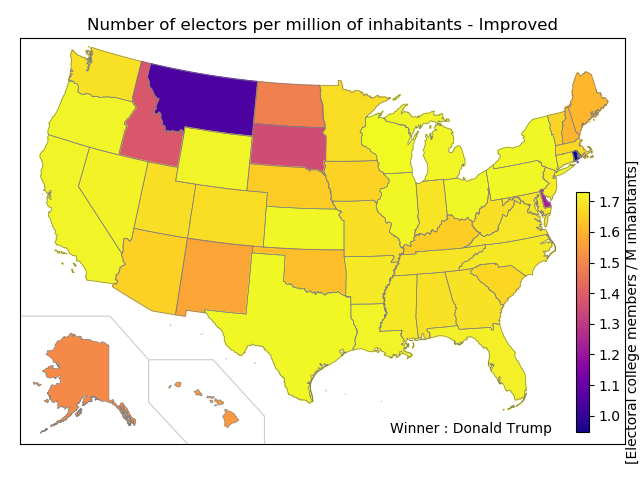
\includegraphics[width=\linewidth]{mapTotalImproved}
	\caption{Distribution with conditioning - Whole population}
\end{figure}


\end{document}